% Hasentiles! Hase = zajíc (D)

\section{Wang-tile models}

\subsection{Definition}
	
	More abstract model where one handles only with ``glues'' on edges of Wang tiles. Define {\em temperature}.

\subsection{Computational power}
	
	Give table of Turing universality \cite{cook_temp1}.
	
	See \cite{winfree_phd}. Many other results in \cite{cook_temp1}, \cite{stage_assembly}, \cite{square_lb}, \cite{square_ub} \ldots
	
	\subsubsection{Turing universality of 2D tiles at $T=2$}
		
		\begin{figure}[H]
		\begin{center}
			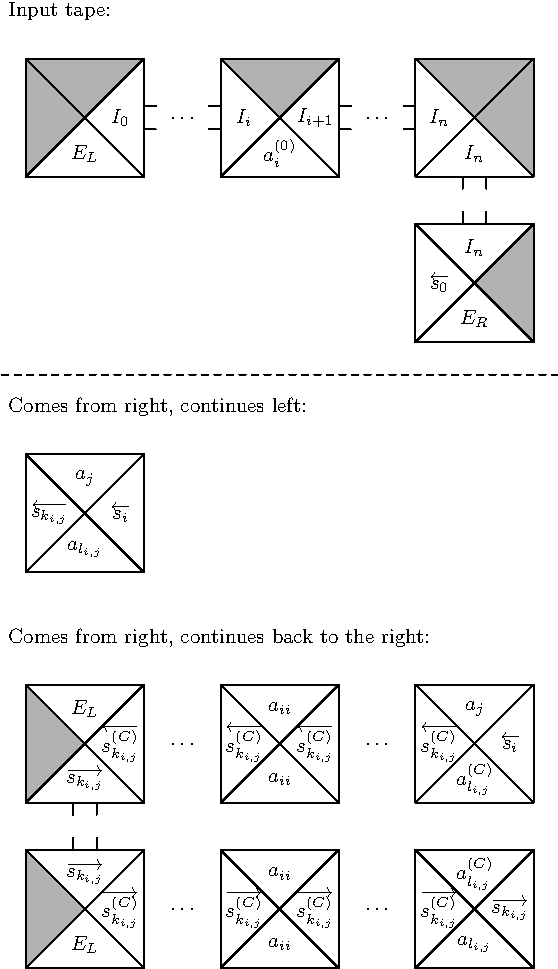
\includegraphics{./figures/tiles1.pdf}
			\caption{Tileset 1/2.}
		\end{center}
		\end{figure}
		
		\begin{figure}[H]
		\begin{center}
			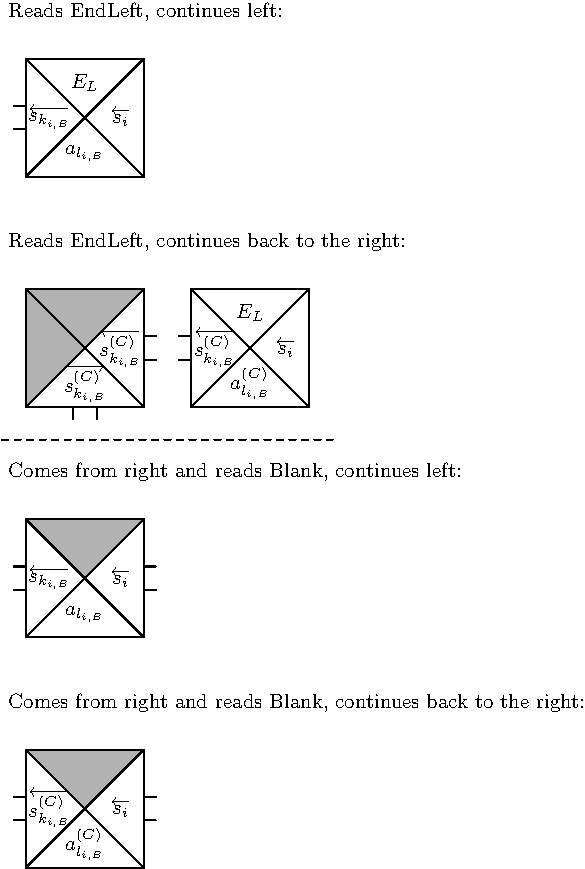
\includegraphics{./figures/tiles2.pdf}
			\caption{Tileset 2/2.}
		\end{center}
		\end{figure}
	
	%%%%%%%%%%%%%%%%%%%%%%%%%%%%%%%%%%%%%%%%%%%%%%%%%%%%%%%%%%%%%%%%%%%%%%
	
	% error-tolerant rules -- Gacs and Reif, 1988\\
